\documentclass[12pt]{article}
\usepackage{amsmath,amssymb,amsthm}
\usepackage{fullpage}
\usepackage{graphicx}
\usepackage{hyperref}
\usepackage{listings}

\theoremstyle{definition}
\newtheorem{thm}{Theorem}[section]
\newtheorem{lem}[thm]{Lemma}
\newtheorem{defn}{Definition}[section]
\newtheorem{conj}{Conjecture}[section]
\newcommand{\floor}[1]{\left\lfloor #1 \right\rfloor}
\newcommand{\ceil}[1]{\left\lceil #1 \right\rceil}
\newcommand{\bigC}[0]{\mathcal{C}}
\begin{document}
\emergencystretch 3em
\title{How hard is it to detect {\em some} cliques?}

\author{Josh Burdick}

\maketitle

\begin{abstract}
Shannon's function-counting argument
\cite{shannon_synthesis_1949} showed that most Boolean functions have
exponential circuit complexity, but doesn't provide a specific example
of such a hard-to-compute function. A simple modification of that argument
shows that detecting a randomly-chosen subset of the $k$-vertex cliques in an
$n$-vertex graph requires, on average, $\Omega(n^{k/2})$ NAND gates.
Unfortunately,
this doesn't directly bound the complexity of detecting {\em all} of the cliques;
however, it seems like a related problem.
Here, we attempt to combine a counting argument with
random restrictions, to estimate the number
of NAND gates needed to detect some cliques (as a function
of the number of cliques).
\end{abstract}

\newpage

\tableofcontents

This is an attempt to obtain a lower bound on the the number of NAND gates
needed to detect {\em some} of the cliques in a graph (as opposed to
all of them).
Although it seems unlikely to work, hopefully
it will add to the long list of strange things which would happen
if P = NP \cite{fenner1996complexity}.

\section{A counting bound}
\label{countingBound}

The first component we use is a slight modification
of Shannon's function-counting argument
\cite{shannon_synthesis_1949}.

\subsection{Background: lower bounds from function counting}

It has long been known that computing {\em some} function of a bit-string
requires exponentially large circuits \cite{shannon_synthesis_1949}.
Let $f: \{0,1\}^m \rightarrow \{0,1\}$ be a function from bitvectors to bits.
If there are $m$ inputs to a circuit,
then there are $2^{2^m}$ possible functions from the $m$-input bitstring to
a one-bit output. Each of these functions, being different, must have a
different circuit.

Given a count of functions, we can then see, for instance,
how many unbounded fan-in NAND gates are needed to compute
those functions (see Theorem \ref{boundFromCounting}
in Appendix \ref{gateMath}).

However, this argument also applies to a subset of the functions defined
on $m$ inputs.

\subsection{Counting CLIQUE-like functions}

In particular, suppose we are given an $n$-vertex graph.
Let $k$-CLIQUE($n$) be the boolean function which
detects $k$-cliques: it outputs 1 if any $k$-clique
is present, and 0 otherwise. This is a classic
NP-complete problem.

We now consider a ``buggy'' variant of the $k$-CLIQUE function,
which only detects a subset of cliques. (Nomenclature note:
technically, since
we're only trying to output a 1 iff there's a clique, I should say
``detects''; ``finding'' a clique would mean outputting its
vertices as well. I'll probably write ``finds'' here for now,
even though it isn't exactly the right nomenclature.)

As a concrete example,
consider the set of ``buggy'' 6-clique detectors.
Maybe the circuit correctly
finds all the cliques. Or maybe it finds all of the cliques except $K_{1..6}$,
or it misses half the cliques, or finds none (and always outputs 0), or maybe
it only successfully finds $K_{1,3,4,5,7,8}$, et cetera.

We define a variant of $k$-CLIQUE which only
finds a subset of cliques.
Let $K$ denote the set of all possible
$k$-vertex cliques.

\begin{defn}
\label{BUGGYCLIQUE}
Let $A \subseteq K$.
Let $m = {n \choose 2}$ be the number of edges in the input graph.
$BUGGYCLIQUE(A): \{0,1\}^m \rightarrow \{0,1\}$ is the function which
is 1 iff any of the $K_k$s in $A$ is present.
That is, for each set $A$ of $K_k$s, $BUGGYCLIQUE(A)$
contains a function which is 1 if the input contains any $K_k \in A$,
and 0 otherwise. (Using this nomenclature,
$k$-CLIQUE(n) = $BUGGYCLIQUE(K)$).
\end{defn}

Of course, many of these functions are quite similar (e.g. all but one of them
output a 1 when you feed in all 1's). However, they're all slightly different.

\begin{thm}
\label{buggyDistinct}
There are  $2^{|K|}$ distinct $BUGGYCLIQUE$ functions.
\end{thm}
\begin{proof}

Let $A,B \subseteq K$, with $A \neq B$, and w.l.o.g.
let $x \in A-B$. Then $BUGGYCLIQUE(A)$ outputs 1 on the input
with just the edges in $x$ set to 1 (and 0 everywhere else),
while $BUGGYCLIQUE(B)$ outputs a 0.

There are $2^{|K|}$ many subsets of $K$,
and by the above, each corresponds to a diffferent function.
\end{proof}

For a given $A$, many of the functions in $BUGGYCLIQUE(A)$
are similar (for instance, most
of them output a 1 when all the edges are present);
but they are all distinct.
Although $2^{n \choose k}$ is a fairly large number,
it's still comfortably less than $2^{2^{n \choose 2}}$, the number of boolean
functions on the ${n \choose 2}$ input wires (one per edge).

\subsubsection{But {\em which} function requires many gates?}

Thus, there are $2^{n \choose k}$ different functions. 
How many NAND gates do these take?
(We consider NAND gate circuits (with any fan-in) which find $k$-cliques in $n$-vertex
graphs, as a circuit with $n \choose 2$ inputs.)

Applying Theorem
\ref{boundFromCounting}, we know that at least one of the circuits requires
${\sqrt {2 {n \choose {k/2}} + b^2}} - b = \Omega(n^{k/2})$ 
NAND gates (where $b = {k \choose 2} - 0.5$).

Why doesn't this bound $k$-CLIQUE?
Because we don't know that the circuit which finds {\em all} of the
$K_k$s is one of these larger circuits. As far as what I've
shown thus far goes, it could be harder to find some weird subset of the $K_k$s.

Indeed, as far as what we've formally shown goes, the problem which needs
the most NAND gates could be finding a single clique! That's easily ruled out
(because that only needs one NAND gate, plus the output gate).

\subsection{Which sets of cliques are hard to find?}
\label{sec:whichCliques}

The hardness of these functions depends
on how the cliques they find are laid out.

Cliques are arguably difficult to draw in a two-dimensional space.
As an approximate diagram reflecting what we know,
we sketch a Hasse diagram of possible subsets of cliques. Although
we only draw a few subsets of three-vertex cliques
on six vertices, hopefully this provides some
intuition.

\begin{figure}
\centering
\includegraphics[width=1\textwidth]{R/Hasse.pdf}
\caption{Hasse diagram of BUGGYCLIQUE functions.
(a-d) 
Detecting all the possible cliques in larger graphs will be
increasingly difficult (although {\em how much} harder isn't clear).
(e) 
Detecting this set of cliques is definitely harder than (b),
since we can convert from (e) to (b) by feeding in 0's to
some set of edges.
(f) Detecting a set of cliques which doesn't overlap much will be
harder than detecting the same number of cliques, when they overlap
maximally (as in (b)).}
\label{fig:Hasse}
\end{figure}


\begin{thm}
\label{edgeZonking}
Let $A \subsetneq B \subseteq K$, such that $A$ is what remains
of $B$ after removing all cliques overlapping some edge $e$.
Then $|\bigC(BUGGYCLIQUE(B))| > |\bigC(BUGGYCLIQUE(A))|$.
\end{thm}
\begin{proof}
Feed in a 0 to $e$, which is in $B$; the remaining cliques are $A$.
The resulting
circuit computes $BUGGYCLIQUE(A)$, and so has size
at least $|\bigC(BUGGYCLIQUE(A))|$. But at least one
NAND gate has been removed by feeding in the 0.
\end{proof}

This shows that sometimes, finding a larger set of cliques is
harder. However, the above theorem doesn't help if the two
sets of cliques cover the same set of edges.

\begin{defn}
\label{zRelation}
Let $A, B \subseteq K$. We define a relation $Z$ (on sets of cliques) :

$Z(A,B)$ iff there is some edge $e$ such that $B$ contains all of the
cliques in $A$ except those which intersect $e$. Thus, $B$ consists
of exactly the cliques in $A$ which would be ``left over'' after
feeding in a 0 to $e$.
\end{defn}

\begin{figure}
\label{Z}
\centering
\includegraphics[width=1\textwidth]{py/figure/Z.png}
\caption{$Z(A,B)$}
\label{fig:Z}
\end{figure}

If we consider $Z(A, B)$ as a relation, then it defines a meet-semilattice
(lower semilattice) with 
many distinct upper bounds.  Indeed, any pair of subsets which
cover all of the input edges are an upper bound, all of which
are incomparable. They thus form an antichain, and so Dilworth's Theorem
implies that these could be formed into chains. Each chain (by construction
of the relation $Z$) has a strictly increasing number of gates, and so the
functions at each level of the chain are strictly increasing in average
size. (However, this doesn't seem to bound the number of gates in CLIQUE.)


Figure \ref{Z} attempts to plot $Z(A,B)$. Using more vertices, or
larger cliques, seems like it would quickly get unmanageable.
Note also that this is ``not to scale'' in a variety of ways. In
particular, when $n$ is large, the middle layer dominates the graph
(because if each clique is chosen with probability 1/2, on average,
you'll pick very close to half the edges).

Each line between sets indicates a set which requires a strictly larger number
of gates.
Unfortunately, at least according to this relation,
the number of sets of cliques smaller than
any of these upper bounds is less than $2^{\# input edges}$.
(For instance, the top levels are only forced to be higher than
a tiny fraction of these sets.)

\begin{figure}
\label{overlappingTris}
\centering
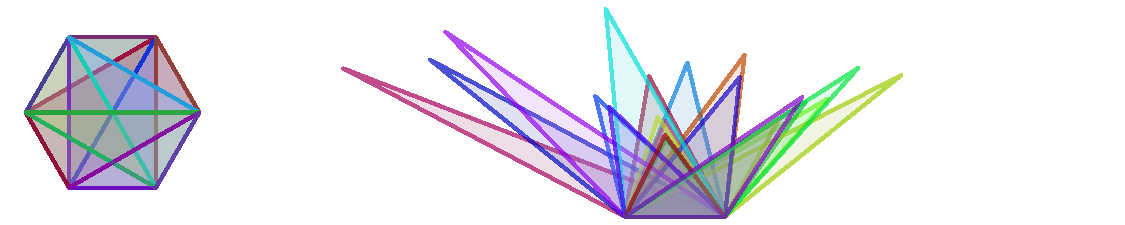
\includegraphics[width=1\textwidth]{R/tri1.pdf}
\caption{A given number of cliques can overlap maximally (left),
or not overlap much (right).}
\label{fig:overlappingTriangles}
\end{figure}

Triangles can be detected using matrix multiplication \cite{itai_finding_1977},
and there are fast algorithms known for matrix multiplication
\cite{strassen_gaussian_1969}
\cite{williams_multiplying_2012}, so the set of all possible
cliques on some set of vertices (Figure \ref{overlappingTris}, left)
 can be detected
using fewer than one NAND gate per triangle (for large enough input graphs).

On the other hand, if the triangles overlap less (as in
Figure \ref{overlappingTris}, right),
then to detect all of the triangles, we will definitely need at least one
gate per triangle. We can see this by feeding in a 0 to some input
unique to a triangle, applying \ref{edgeZonking}, and repeating.

Consider the case of finding $k$-cliques on $n$ vertices.
Possibly the most na\"ive strategy in this case is to pick a vertex $v_1$,
and feed in 0's to edges, one at a time. We can repeat this
(zonking at least one NAND gate as we go), until there
$k-2$ edges remaining connected to $v_1$. At this point, $v_1$ can no
longer be part of a clique. We feed in 0's to those edges (with no
provable effect on the circuit size), and repeat with $v_2$...
This strategy is simple, but only gives a bound a bit lower than
the number of input edges.

\subsection{Defining levels of CLIQUE}

To me, it seems a reasonably intuitive guess that the hardness of
computing $BUGGYCLIQUE(A)$ should be somehow related to
$|A|$, which is simply the number of cliques it ``sees''.

\begin{defn}
\label{CLIQUE-level}
Assume $n, k$ are fixed. For any $l$ such that
$0 \le l \le |K|$, let $K_l$ be the set of all sets
with exactly $l$ cliques. 
\end{defn}

We abuse notation slightly, and write

\[
BUGGYCLIQUE(K_l) = \{ BUGGYCLIQUE(k) : k \in K_l \}
\]

What can we say about $E[|\bigC(BUGGYCLIQUE(K_l))|]$, for
some fixed $l$? Let $N = {n \choose k}$.
At the ``bottom'', there's only one $BUGGYCLIQUE(\emptyset)$
function, so the counting argument is useless.
In the ``middle'',
there are ${N \choose {N/2}}$ functions, and so the counting
argument gives a nontrivial lower bound for
$E[|\bigC(BUGGYCLIQUE(K_{N \choose {N/2}}))|]$ (although
without actually constructing even {\em one} difficult function!).
At the ``top'', again, there's only one $BUGGYCLIQUE(K) = k-CLIQUE$
function, so the counting argument is, once again, useless.

It would be nice if we could show that, as $l$ increases,
$E[|\bigC(BUGGYCLIQUE(K_l))|]$ also increases.
If we could prove something in general, for all levels $l$, then at
the top of the diagram, we'd be bounding just the function
$BUGGYCLIQUE(K_l) = k-CLIQUE$. (This suggests that doing so would
be difficult...)


\section{Using random restrictions}

Random restrictions have been used in lower bounds of formula
\cite{subbotovskaya1963comparison} and circuit \cite{hastad1987lower}
complexity (see also the slides at \cite{rossmanRestrictions}).
Here, we apply random restrictions to a set of functions (and circuits),
rather than just one function and circuit.

??? Is this just a ``gate-elimination argument''?

\subsection{Counting functions by their ``rank'' in a list}

This argument relies on measuring the size of a circuit,
for a given basis. (Here, we assume unbounded fan-in
NAND gates, but this doesn't seem crucial.)

\begin{defn}
\label{Rank}
For all $C \subseteq K$,
arrange all of the sets of cliques in nondecreasing order
of $|\bigC(BUGGYCLIQUE(C))|$ (using unbounded fan-in NAND gates,
breaking ties by some lexicographic order of circuits).

Let $A \subset K$. The {\em rank} of $A$, $rank(A)$, is the zero-based
index of $A$ in this list.
\end{defn}

If we can lower-bound $rank(A)$, then we should be able to translate
that into a
lower bound on $|\bigC(BUGGYCLIQUE(A))|$. (Possibly, if we
can only lower-bound $E[rank(A)]$, we may be able to get
a bound in terms of number of gates using Jensen's inequality?
Not clear.)

We can imagine a miles-long linear warehouse of chips with the minimal
circuit for each problem, sorted in terms of number of gates.
Note that the above list only includes functions in $BUGGYCLIQUE$.
There are a {\em ton} of other functions (parity, primality, ``looks
sort of like a bitmap of a cat'', etc.), but ignoring
those should still leave a valid lower bound for the functions in $BUGGYCLIQUE$.

\subsection{How much smaller are ``restricted'' circuits, on average?}

\begin{thm}
\label{vaguelyUpward}
Let $C \subseteq K$ be a set of cliques chosen uniformly at random
from $K$.

Let $a = {n-2 \choose k-2}$ (this is the number of $k$-cliques
intersecting a given edge).

Then there is a function $f: 2^K \rightarrow 2^K$ such that
\begin{itemize}

\item $E[|C| - |f(C)|] = a/2$

\item $E[rank(C) - rank(f(C))] = a/2$

\end{itemize}

\end{thm}
\begin{proof}

Pick a distinguished input edge $e$, and let $A \subseteq C$ be
the set of cliques in $C$ which include $e$, and $B \subseteq C$ be
the set of cliques in $C$ which don't include $e$.

We define $f(C) = B$.

Now, take the circuit computing $BUGGYCLIQUE(C)$, and
feed in a 0 to $e$. The resulting circuit computes
$BUGGYCLIQUE(B)$. Note that $A$ could contain anywhere
from 0 to $a$
cliques, so since $C$ is chosen uniformly at random,
$E[|A|] = a/2$.

Furthermore, $|\bigC(B)| \le |\bigC(C)|$, because feeding in
a zero to the circuit for $BUGGYCLIQUE(C)$ constructed a
(possibly non-optimal) circuit for $BUGGYCLIQUE(B)$.
Thus, $rank(B) \le rank(C)$.
This means that
$C$ is one of $a$ functions chosen uniformly at random,
and so, on average, there are $a/2$ circuits between $C$
and $B$, implying at least that large a difference in rank.

(Note that if $e$ ``misses'' all of the cliques in $C$, then $B = C$
and $rank(B) = rank(C)$. However, provided $e$ is in some clique in $C$,
then since we're feeding in a 0 to a NAND-gate circuit,
the inequality $rank(B) < rank(C)$ is strict.)

\end{proof}

In terms of the previous warehouse analogy, we can imagine that,
when an edge is disabled, the chip now has strictly fewer gates.
Perhaps the chip-maker spent their entire budget on designing the
optimal circuits, but then skimped on the wires connecting the chips?
In that case, assuming the missing wire is treated as a 0, the chip still
finds some cliques, and so might yet be sellable.
By construction of the warehouse, that means the faulty chip could be shifted,
on a giant conveyor belt,
toward the ``smaller'' (in number of gates) end of the warehouse.
That means that the corresponding set of cliques is also
in the ``smaller'' end of the warehouse.

Although both these numbers (the reduction in number of cliques, and
the reduction in rank) have an expected value of $a/2$,
they aren't necessarily the same, or even correlated.
(Indeed, when $n$ is large, the number of cliques is sharply peaked around $a/2$,
but the lower bound in reduction in rank is uniformly distributed across $0..a$.)

\subsubsection{Why this doesn't bound $k-CLIQUE$?}

\ref{vaguelyUpward} seems to show that ``finding more cliques is
at least a tiny bit harder on average.'' However, it only applies
on average.

What happens if we try to use restrictions to bound $k-CLIQUE$?
If we start ``at the top'',
feeding in a 0 to $k-CLIQUE$, which is one function,
we get only one other function.

However, it seems vaguely plausible to proceed ``bottom-up'',
estimating the difficulty of finding increasingly large
sets of cliques.

\subsection{Estimating the rank of functions, at each level}

It seems intuitive that finding a larger fraction of the cliques
should be harder.
So, another idea is to try to show this using induction on $l$.
As usual, the base case ($l=0$) is easy: finding zero cliques is easiest,
so its rank is 0.

The step case is not so straightforward. Suppose we've computed bounds for
levels 0 through $l-1$ (thus, we're using some sort of strong induction.)
In other words, we've lower-bounded $E[rank(K_i)]$, for $i \in [0,l-1]$.
Can we lower-bound $E[rank(K_l)]$?

Suppose we pick a set of cliques at level $l$, uniformly at random.
If we then pick an edge $e$ uniformly at random, and remove the cliques
which contain $e$, then the number of cliques removed will vary
depending on the level. When $l=1$, we'll remove 0 or 1 cliques; when $l=N$,
we'll remove all ${n-2 \choose k-2}$ cliques which contain $e$.

We can {\em estimate} the number of cliques removed, by supposing that each
clique is ``hit'' by $e$, with probability $p = {k \choose 2} / {n \choose 2}$.
If we assume that $e$ hitting each clique is an independent event, then
restricting a random set of $l$ cliques will hit $pl$ cliques, and
leave $(1-p)l$ cliques.
In general, when $n>>k$, $p$ will be pretty small. Thus, the step case at
level $l$ will depend on estimates for levels fairly ``high up'' near $l$.
Also, when $n$ is large, $N$ is way larger; so the distribution of
the fraction of cliques removed will be sharply peaked near $p$.

However, this induction isn't quite correct.
We may have a bound on $E[rank(K_i)]$, for $i$ in $[0,l-1]$.
But when we pick a random set of cliques $K_l$, and feed in a 0, we definitely
aren't sampling uniformly from levels 0 through $l-1$, because the graphs we're
sampling definitely lack one edge.

Thus, this is {\em only an estimate} of the rank of functions at level $l$.
To me, this raises (at least) the following questions:

\begin{itemize}

\item If we compute the estimate, what do we get?

\item Is there a way to modify this, to get an actual bound?

\end{itemize}

I only address the first question, and punt on the second.

\subsection{An estimated bound}

Thus, even though this is an estimate, we ``simulate'' this process, starting
at level 0, and going up to level $N = {n \choose k}$. 
First, define $p$, the estimated probability that a 0 ``hits'' a clique:

\[ p = \frac{{k \choose 2}}{{n \choose 2}} \]

Assume that the number of cliques after feeding in a 0 follows a binomial
distribution, with $l$ ``trials'' and ``probability of success'' $1-p$.
$B(l)$ will then be a weighted average of $B(0)$ through $B(l-1)$. However,
if the 0 ``misses'' all the cliques, then we can't say anything about the
rank, and just use 0.
Furthermore, we know that at level $l$, we're adding ${N \choose l}$ new
functions.


Let $R(l)$ be the lower bound on the expected rank of functions in $K_l$.

\[
R(0) = 0
\]

For $0 < l \le N$, define
\[
	R(l) = [ \sum_{1\le i < N} binom(i; l, 1-p) R(i) ] + {N \choose l}/2
\]

The file {\tt py/approxRank.py} computes this bound. However, as noted above, this
is only an approximation, because after you feed in a 0, you're no longer
{\em uniformly} sampling from smaller sets of cliques.

\subsection{Description of an attempt to remedy this}

{\tt py/lp\_gate\_bound.py} is an attempt to remedy these problems.
It formulates the lower bound as a linear programming (LP) problem,
with a variable for problems with various numbers of cliques.
It counts the bounds in terms of ``number of two-input NAND gates''.

For a given set of cliques $C$, it divides these into the cliques
hit by zeroing an arbitrary random edge, and those remaining.
Let $n$ be the number of vertices, and $k$ be the size of the clique,
and $N = {n \choose k}$ be the number of cliques. Then zeroing
an arbitrarily-chosen edge could potentially eliminate up to
${n-2 \choose k-2}$ cliques.

Concretely, if $n=9$ and $k=3$, then there are 84 possible 3-cliques
(triangles), and zeroing out an arbitrarily-chosen edge could
eliminate up to 7 of these cliques.

\subsubsection{Equality constraints}

(added by {\tt lp.add\_total\_cliques\_equality\_constraints()})

For some parts of this attempt, we need to think in terms of
the total number of cliques. For other parts, we need to pay attention
to how many cliques are ``hit'' by the zeroed edge. This constraint
relates these: the cost of finding some set of cliques, is an
average, weighted by how many cliques are ``hit'' by a random edge.

\subsubsection{Counting-bound constraints}

(added by {\tt lp.add\_total\_cliques\_counting\_bound\_constraints()})

This includes the actual counting bound. Specifically, for
each total number of cliques, this counts the number of functions,
and constrains the expected number of gates.

\subsubsection{Zeroing constraints}

(added by {\tt lp.add\_edge\_zeroing\_constraints()})

These encode the fact that if you feed in a 0 to an edge,
you will end up with a circuit which finds a strictly smaller
set of cliques. Note that we're only guaranteed that this
number is 1 less.

\subsubsection{Upper bound}

(added by {\tt lp.add\_upper\_bound\_constraints()}, if you give
the {\tt --upper-bound} command-line flag)

This encodes an {\em upper} bound.
Let $C$ be a set of cliques, and suppose we divide $C$ into
disjoint sets of cliques $A$ and $B$. Given circuits to
find those sets of cliques, we can clearly find the cliques
in $C$ by OR'ing those together. Implementing 2-input OR can be
done with three 2-input NAND gates. Thus, on average, we have

\[
|\bigC(C)| \le |\bigC(A)| + |\bigC(B)| + 3
\]

It may seem weird to include an {\em upper} bound. What was
my motivation? My thinking was that this might connect the difficulties
of finding cliques at each ``level''. As noted earlier, CLIQUE
is only above a fraction of the sets in $Z$. When the LP solver
``pushes down'' on CLIQUE, it also pushes down on that rather small
set. But (my thinking was), with this upper bound, some of the
higher-up sets would also be ``pulled down''; hopefully they'd
eventually run into the counting bound. That is admittedly
not a rigorous description.

\subsection{Results}

Here is what this model estimates. Note that this quickly starts
to be solving humungous LP problems. (Exercise for the reader:
how many variables does this use, to model finding $k$-vertex
cliques in an $n$-vertex graph?)

\begin{verbatim}
$ ./lp_gate_bound.py 7 3
30.7092
$ ./lp_gate_bound.py 7 3 --include-upper-bound
13.213
$ ./lp_gate_bound.py 8 3
34.6822
$ ./lp_gate_bound.py 8 3 --include-upper-bound
21.6523
$ ./lp_gate_bound.py 9 3
34.6545
$ ./lp_gate_bound.py 9 3 --include-upper-bound
51.5385
\end{verbatim}

\subsection{Further thoughts on this model}

Having implemented this, and somewhat attempted to describe it,
I'm contemplating major revisions.

The idea of bounding the ``rank'' of functions (as in the
``miles-long linear warehouse'' model) seems massively cleaner to reason about.
Dealing with the nitty-gritty of converting from ``number of functions''
to ``number of 2-input NAND gates'' is complicated. The motivation
for doing this was that it simplified adding an upper bound.
However, in the rank model, we could simply bound the
average cost of finding a uniformly-randomly-chosen set of cliques, as
${n \choose k}/2$. This bound is exact (in other words, both an
upper and lower bound).

Also, zeroing out a random edge seems to complicate the book-keeping,
as after doing so, you can end up with an arbitrary weird set of
input edges left over. It seems (retrospectively) much simpler to
simply feed in 0's to all the edges incident to an arbitrary vertex.
You then always end up with a graph with one less vertex.

Various other files in the {\tt py/} folder implement attempts at
this, without much success; but I may revisit those.

\section{Related work}

This strategy relies heavily on a modification of Shannon's original
function-counting argument \cite{shannon_synthesis_1949},
combined with random restrictions
\cite{subbotovskaya1963comparison} \cite{hastad1987lower}.

A related question is whether problems
(such as $k$-SAT) are
hard on average \cite{bogdanov2006average}.
These efforts seem to focus more on whether
random
instances of a given problem are hard, rather
than using random problems to show that
a specific problem is hard.

??? What about:
- co-NP?
- formula size?


This lower-bound strategy also seems potentially
relevant to quantum computing,
as the argument makes few restrictions on the sort of gates used.
However, we did use the property of NAND gates that ``feeding in
a 0 disables a gate''; it's not clear whether that's needed,
or holds for quantum gates.

\section{Conclusion}

We give a lower bound on finding {\em some} set of cliques.
It is a modified form of Shannon's counting argument
\cite{shannon_synthesis_1949}, combined with random restrictions
\cite{subbotovskaya1963comparison} \cite{hastad1987lower}.
This suggests {\em approximate} bounds on functions {\em similar} to $k$-CLIQUE.
Unfortunately, however, this is an approximate bound,
and so doesn't bound the complexity of $k$-CLIQUE.

If this worked, then by the contrapositive,
\cite{fenner1996complexity} would give a concise list of some of the consequences...

\section{Acknowledgements}

The author would like to thank William Gasarch for introducing him
to lower bound strategies, and probabilistic proofs.
He would also like to thank the maintainers of
several entertaining and relevant blogs, including but
not limited to: the Computational Complexity blog
(Lance Fortnow and William Gasarch), 
G\"odel's Lost Letter (Richard Lipton and Ken Regan),
and Shtetl-Optimized (Scott Aaronson). 


\appendix
\section{Calculations for unbounded fan-in NAND gates}
\label{gateMath}

We used unbounded fan-in NAND gates largely because they are
convenient to convert from ``number of functions'' to
``number of gates''.

Let $\bigC(f)$ be the circuit
with the fewest unbounded fan-in NAND
gates computing $f$, and let $|\bigC(f)| = g$ be the number of gates in
that circuit. The
circuit could have at most $gm$ wires from inputs to gates, and ${g \choose 2}$
wires from gates to gates. We can view the possible circuits as a bitmask,
containing a 1 everywhere a gate is connected to an input (or another gate),
and 0 everywhere else.

\begin{thm}
\label{boundFromCounting}
Consider functions from $m$ bits to one bit of output.
This means that, with $g$ gates, we can represent at most
$2^{gm + {g \choose 2}}$ different boolean functions (with $m$ bits of input,
and one bit of output).
\end{thm}
\begin{proof}

The number of possible wires which are there, or not, is $gm + {g \choose 2}$,
which bounds how many possible circuits there are.
Some of these circuits compute the same function.
However, there can't be any more than this many circuits with this many wires.
\end{proof}

This means that if we have a large set of functions, and we know the size of
the set of functions, then we know that at least {\em one} of them requires
a large number of gates. (Knowing {\em which} function requires a lot, or many,
gates is still an issue).

We used unbounded-fan-in NAND gates because, given a number of circuits,
it's easier (I think!) to solve for the number of wires than if we had
used two-input gates.
Consider functions from $m$ bits to one bit of output.
Let $g$ be the number of gates, and $w$ be the number of wires.
Solving for the number of gates:

\begin{eqnarray*}
w & = & mg + {g \choose 2} \\
  & = & mg + g(g-1)/2 \\
  & = & mg + (g^2 - g) / 2 \\
  & = & 0.5g^2 + (m-0.5)g \\
0 & = & 0.5g^2 + (m-0.5)g - w \\
\end{eqnarray*}

We solve the quadratic formula (writing $b = m-0.5$ for simplicity), keeping
only the non-imaginary root.

\begin{eqnarray*}
g & = & -b \pm \sqrt{ b^2 + 2w} \\
  & = & {\sqrt {2w + b^2}} - b \\
\end{eqnarray*}

Thus, given a set of functions, we know that at least one of them requires
this many gates.

This expression is a bit inconvenient, and as $n$ increases, we
expect the number of gates to be much larger than the number of
inputs $b$. To avoid such issues, we can count the number of gates
beyond the number of inputs. This gives the bound

\begin{eqnarray*}
	g & \ge & \sqrt{2w} - m \\
\end{eqnarray*}


\bibliography{references}
\bibliographystyle{unsrt}

\end{document}

